\documentclass[10pt]{IEEEtran}

\usepackage[hyphens]{url}
\usepackage[pdftex,bookmarksnumbered,hidelinks,breaklinks]{hyperref}
\usepackage{amssymb}
\usepackage{amsmath}
\usepackage{caption}
\usepackage{amsrefs}
\usepackage{courier}
\usepackage{graphicx}
\usepackage{bookman}
\usepackage{amsthm}
\usepackage{verbatim}
\usepackage{xcolor}
\usepackage{setspace}
\usepackage{float}
\usepackage{url}
\usepackage{listings}
%\usepackage{appendix}
\usepackage[margin=1in]{geometry}
\bibliographystyle{amsmath}
\newtheorem{definition}{Definition}
\newtheorem{theorem}{Theorem}
\newcommand{\?}{\stackrel{?}{=}}
\begin{document}

\title{Optimization of CUDA-based $n$-Body Simulation}
\date{}
\author{Tyler Allen}
\maketitle

\begin{abstract}
\end{abstract}

\section{Introduction}

\section{Methodology}
\subsection{Implementation}
The $n$-body simulation was written in C++11 and CUDA. Bodies are implemented
with the following elements: a $3$-D position vector, a $3$-D velocity vector,
a $3$-D acceleration vector, and mass. These elements are required portions of
the $n$-body algorithm\cite{meyer}. The initial implementation represents
bodies using C++ objects. The calculation for force applied to body $i$
by all other bodies in one unit of time is presented below\cite{meyer}:
\begin{figure}[H]
\begin{center}
$F_{i} = \sum_{j=1, i\neq j}^{N}\frac{Gm_im_j(p_j - p_i)}{||p_j - p_i||^3}$
\end{center}
\caption{Equation for force applied to body $i$ by all other bodies.}
\label{nbody}
\end{figure}
This formulation includes position vectors represented by $p$, mass represented
by $m$, and a gravitational constant represented by $G$. The output of this
equation is force, which is trivially converted to acceleration since mass 
is known. For each timestep, acceleration can be used to find velocity and 
then position. The value used for for parameter $G$ is $6.674 \times 10^{-11}$\cite{meyer}.
An additional factor, $\epsilon$, has been included as an additive constant
to the magnitude of the distance between two bodies seen in figure \ref{nbody}\cite{nvidia}. 
This factor is to prevent the force calculation from approaching infinity when
objects overlap. The value of $\epsilon$ used in our simulation is 
$\frac{1}{16}$. This value is based on the results of the visualization of the 
$n$-body algorithm, discussed later in this section.

The $n$-body algorithm was implemented as a brute-force solution derived from the
equation in figure \ref{nbody}. This is
primarily because the $n$-body problem is highly parallelizable. This paper
does not focus on more advanced solutions to the $n$-body problem, such as the 
Barnes-Hut algorithm\cite{barneshut}, since this paper is focused  
on CUDA optimizations to an existing algorithm. The algorithm is implemented
as two seperate CUDA kernels. The first kernel, \texttt{calculate\_force},
calculates the force (acceleration) applied to each body during one time step.
The second kernel, \texttt{update\_pos} updates the velocity and position values 
of each body according to their new acceleration. The kernels are split because
\texttt{calculate\_force} has a data dependency on the current position of each
body. Allowing a position update before all new acceleration values have been
calculated would cause some small computation errors. The \texttt{calculate\_force}
and \texttt{update\_pos} functions can be seen in appendix \ref{appendix:calc_force}
and \ref{appendix:up_pos}.

A visualization for the $n$-body problem is contained within this implementation.
The visualization is written using OpenGL\cite{opengl} and using the window 
utility library GLFW\cite{glfw}. The visualization shows each body as a white
particle on the screen. Interactions are not limited in any way, and will 
render as fast as the computation will allow them to. The visualization is 
disabled for all calculations and tests in the remainder of this paper because it 
eventually becomes a bottleneck for the simulation. Figure \ref{vis} contains a screenshot of the
visualization.

\begin{figure}
\begin{center}
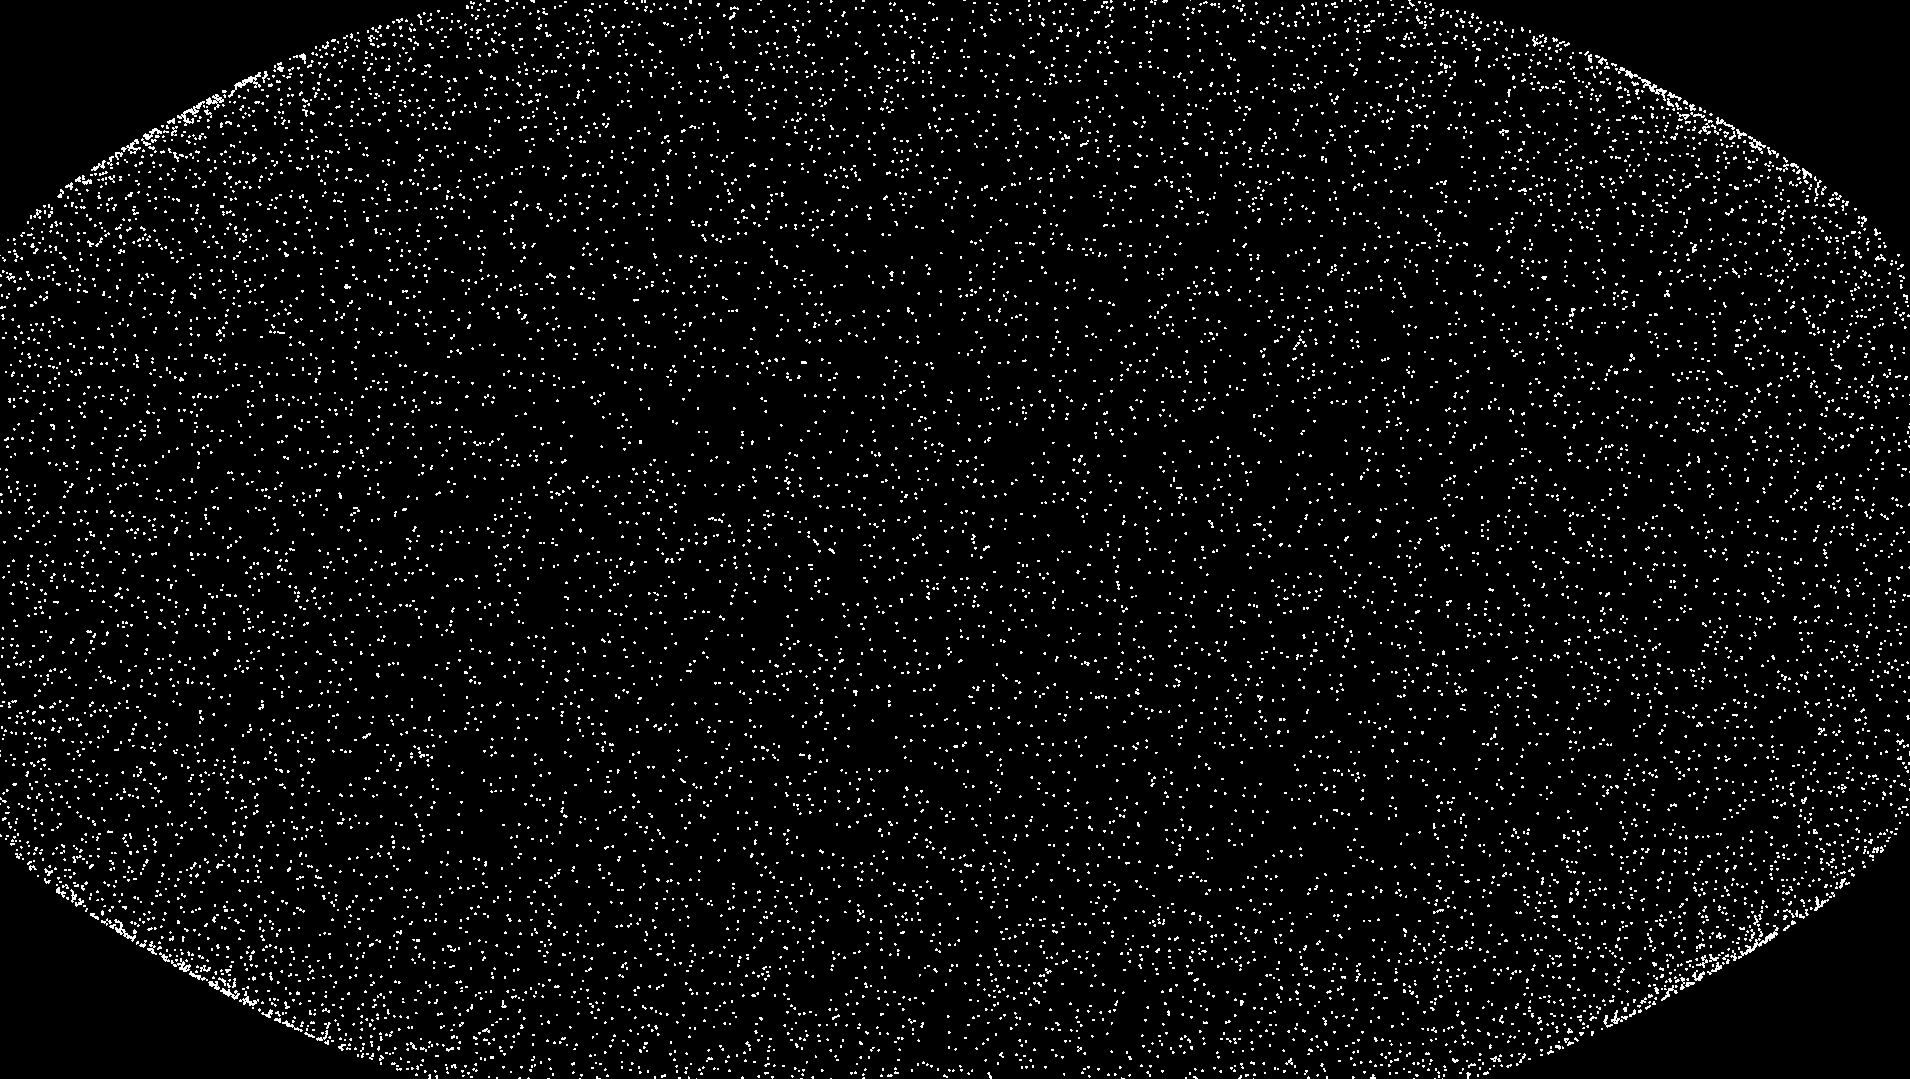
\includegraphics[scale=.12]{vis.png}
\caption{A screenshot of the $n$-body visualization rendering $16384$ bodies.}
\label{vis}
\end{center}
\end{figure}

\subsection{Testing Conditions}
The testing conditions and performance metrics will be described here. We will
rate the performance of an individual run of the simulation using ``frames''. 
A frame is one full iteration of the main loop. The main loop contains the two
CUDA kernels mentioned previously, as well as a memory transfer of position 
data to main memory from the device. Frames are used because this optimization
will be focused around generating data for a specific use case, such as rendering.
Therefore, each ``frame'' requires the transfer of data back to main memory. As
previously mentioned, the rendering is not part of the test. To account for this,
we will procede under the assumption that visualization is able to be rendered
``infinitely fast,'' and that the rendering does not require any computational
resources provided the position data is present in main memory after each 
iteration.

Other metrics may also be used to describe performance where relevant, such as 
locality or occupancy. These metrics are provided by profiling tools described
in the next section. Since these profiling tools affect the performance of 
the simulation, these metrics will not be taken from the same simulation runs
as the frames metric is taken. Instead, frames will have several non-profiled 
runs from which the average frame count will be derived, and then profiled runs
 will be performed.

Every simulation will be $60$ seconds long. Time is kept on an 
internal timer within the main loop. Therefore time may add bias against implementations
with greater performance by slowing the main loop down for each iteration. We will
show this bias is minimal. An external clock could have been used but may have
been unreliable for stopping the program at the appropriate time. This would
have also introduced a degree of bias.

The number of bodies used in the experiment will be stated for each test case. 
The number of bodies changes because the initial implementation was too slow to
render any larger number of bodies. In order to maintain the frame of 
reference, a comparison will be made between the same implementation at higher
number of bodies when the number of bodies increases. 


\subsection{Performance Optimization}
In this section we will described the tools used for optimization, as well 
as the optimization techniques used. These optimization techniques are general
techniques for improving performance. The next section will focus on optimizations
targeting specific hardware and CUDA versions for improving performance across
different GPU hardware. We focus soley on the time spent in the main loop of 
the simulation, so time spent in initialization and finalization is not a concern
of this paper. The areas of optimization that received focus are GPU parameters,
memory organization and allocation, numerical and branch operations within 
CUDA kernels, type optimizations, and optimization flags.

In order to gauge the performance of the program and identify possible areas
for improvement, several profiling tools were used. These profiling tools 
include \texttt{gperftools}\cite{gperftools}, NVIDIA \texttt{nvprof}\cite{nvprof}, and NVIDIA 
NSight\cite{nsight}. \texttt{gperftools} is a CPU profiler. For the purpose
of our simulation, its purpose is to identify CPU-based bottlenecks within the
main program segment. We use this tool to help mitigate the CPU's impact on the CUDA-based
code to improve the accuracy of performance data. NVIDIA NSight is a visual
profiling tool for profiling GPU usage. It includes information such as the 
amount of program time spent executing each kernel, locality information,
and device/host memory transfer time. It also provides performance analysis 
information to guide the user towards areas that can be optimized. We use this 
tool to acquire metrics on our CUDA kernels that we can attempt to improve.
\texttt{nvprof} provides the same primary functions as NSight, but it is a 
command line based tool.

\subsection{GPU-based Optimization}
In this section we will describe the CUDA parameters used to optimize the 
simulation for different hardware, as well as the hardware used in our test
cases. The primary tool available for this 
optimization is the \texttt{\_\_launch\_bounds\_\_}\cite{bounds}. This function uses the 
arguments \texttt{maxThreadsPerBlock} and \texttt{minBlocksPerMultiprocessor}
to determine the appropriate number of registers to allocate per thread\cite{bounds}. The
maximum values for these two parameters are dependant on the CUDA version 
being used. In the test studies, the number of blocks argument passed to each
CUDA kernel is always the same value as \texttt{maxThreadsPerBlock}, except
in the one case where we do not use the \texttt{\_\_launch\_bounds\_\_}\cite{bounds}.
This will be discussed further in the Results section.

For our test cases, the following GPUs were acquired: a GTX $680$, a GTX $780$M, 
and a GTX TITAN Black. The GTX $680$ and GTX TITAN Black are standard commodity
desktop dedicated graphics cards. The $780$M is a dedicate graphics card for 
laptops. The machines running the $680$ and $780$M run Arch Linux with kernel
version $4.2.5-1$, and the machine containing the TITAN Black runs Ubuntu with 
kernel version $3.13.0$. Each machine had the standard NVIDIA drivers, and 
all code was compiled on each respective machine using the \texttt{nvcc} compiler
from the current CUDA $7.5$ release. It should be noted that the $680$ and $780$M
were imaged by this author and have no limitations set on GPU usage. The author
did not have root access or image information on the computer containing the 
TITAN Black.

\section{Results}
\subsection{Performance Optimization}
\subsection{GPU-based Optimization}

\section{Conclusion}
\subsection{Future Work}

\newpage
\bibliography{report}
\nocite{*}
\newpage
\begin{appendices}
\onecolumn
\footnotesize
\section{Force Calculation Kernel}
\label{appendix:calc_force}
\begin{lstlisting}[language=C++]
extern "C" __global__
void calculate_force(int nbodies, Body* g_bodies, double timestep)
{
    double dx;
    double dy;
    double dz;
    double dist;
    double mass;
    // Current body
    int i = threadIdx.x + blockIdx.x * blockDim.x;
    // For all bodies
    for (int j = 0; j < nbodies; j++)
    {
        // skip self
        if (i != j)
        {
            // change in position, data dependency here
            dx = g_bodies[j].get_pos(0) - g_bodies[i].get_pos(0);
            dy = g_bodies[j].get_pos(1) - g_bodies[i].get_pos(1);
            dz = g_bodies[j].get_pos(2) - g_bodies[i].get_pos(2);

            dist = sqrt(dx * dx + dy * dy + dz * dz);
            dist = dist * dist * dist;
            dist = dist > 1 ? dist : 1;
            //omit mass of current body, must divide by it later to get accel anyway
            mass = timestep * G * g_bodies[j].get_mass();
            g_bodies[i].update_acc(0, mass * dx / dist);
            g_bodies[i].update_acc(1, mass * dy / dist);
            g_bodies[i].update_acc(2, mass * dz / dist);
        }
    }
}
\end{lstlisting}

\section{Force Calculation Kernel}
\label{appendix:up_pos}
\begin{lstlisting}[language=C++]
extern "C" __global__
void update_pos(int nbodies, Body* g_bodies)
{
    int i = threadIdx.x + blockIdx.x * blockDim.x;
    g_bodies[i].update_vel(0, g_bodies[i].get_acc(0));
    g_bodies[i].update_vel(1, g_bodies[i].get_acc(1));
    g_bodies[i].update_vel(2, g_bodies[i].get_acc(2));
    g_bodies[i].update_pos(0, g_bodies[i].get_vel(0));
    g_bodies[i].update_pos(1, g_bodies[i].get_vel(1));
    g_bodies[i].update_pos(2, g_bodies[i].get_vel(2));
}
\end{lstlisting}

\end{appendices}

\end{document}

